%----------------------------------------------------------------------------------------
%    PACKAGES AND THEMES
%----------------------------------------------------------------------------------------

\documentclass[aspectratio=169,xcolor=dvipsnames]{beamer}
\usetheme{SimpleDarkBlue}

\usepackage{hyperref}
\usepackage{graphicx} % Allows including images
\usepackage{booktabs} % Allows the use of \toprule, \midrule and \bottomrule in tables
\usepackage[absolute,overlay]{textpos}

% \usepackage{minted}

\usepackage{xcolor}

\usepackage{adjustbox}
\usepackage{verbatim}
% \usepackage{resizebox}


\usepackage{tikz}
\usepackage{circuitikz}
\usetikzlibrary{arrows.meta, positioning}

% \usepackage[style=numeric-comp,backend=biber]{biblatex}
% \addbibresource{reference.bib}

\newcommand\myheading[1]{%
  \par\bigskip
  {\Large\bfseries#1}\par\smallskip}

% anything surronded by this new command will not do anything
\newcommand{\mycomment}[1]{}
\setbeamertemplate{bibliography item}{[\arabic{enumiv}]}
%----------------------------------------------------------------------------------------
%    TITLE PAGE
%----------------------------------------------------------------------------------------

\title{Real-Time Hyperspectral Signal Processing and Classification}
\subtitle{2025 Final Presentation}

\author{Nash Rickert}

\institute
{
    Electrical and Computer Engineering Department, REU \\
    Montana State University % Your institution for the title page
}
\date{\today} % Date, can be changed to a custom date

%----------------------------------------------------------------------------------------
%    PRESENTATION SLIDES
%----------------------------------------------------------------------------------------

% TODO: Add some image/presentation citations. Practice presentation and write any notes I feel are important to structure the flow of the presentation
\begin{document}

\begin{frame}
    % Print the title page as the first slide
    \titlepage
\end{frame}

%------------------------------------------------
% \section{First Section}
%------------------------------------------------
\begin{frame}{Introduction}
    \myheading{Overview}
    \begin{itemize}
        \item Our goal is to implement \textbf{real-time hyperspectral classification}. This means that our model would be integrated with the data-collection process so that there is no need to handle large amounts of data after collection.
              \begin{itemize}
                  \item Currently it is often the case that large amounts of hyperspectral data will be collected in the field, then need to be processed seperately before any results can be acted upon.
              \end{itemize}
        \item This naturally means that the main goal of our project is to minimize the latency of the classification process so it matches the pace of data collection.
    \end{itemize}

    % Contrast this goal with what typically happens
    \begin{block}{Motivation}
        Real-time classification would provide immediate insight to field workers, allowing them to make important decisions quickly.
    \end{block}
\end{frame}

\begin{frame}{Background: Hyperspectral Imaging (HSI)}
    \begin{columns}
        \begin{column}{0.48\textwidth}
            \begin{itemize}
                \item HSI uses diffraction to sample a continuous range of spectral bands.
                \item Because of its high dimensionality, hyperspectral data tends to be large and difficult to process.
                      \begin{itemize}
                          \item A typical RGB image has 3 channels. Our sensor uses 1608. 535x larger.
                      \end{itemize}
            \end{itemize}
            \begin{figure}
                \centering
                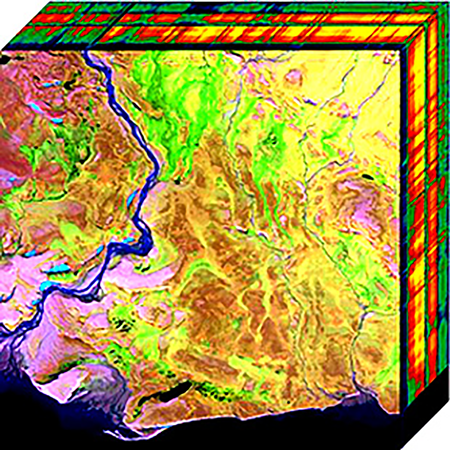
\includegraphics[width=0.5\textwidth]{datacube.png}
            \end{figure}
        \end{column}
        \begin{column}{0.48\textwidth}
            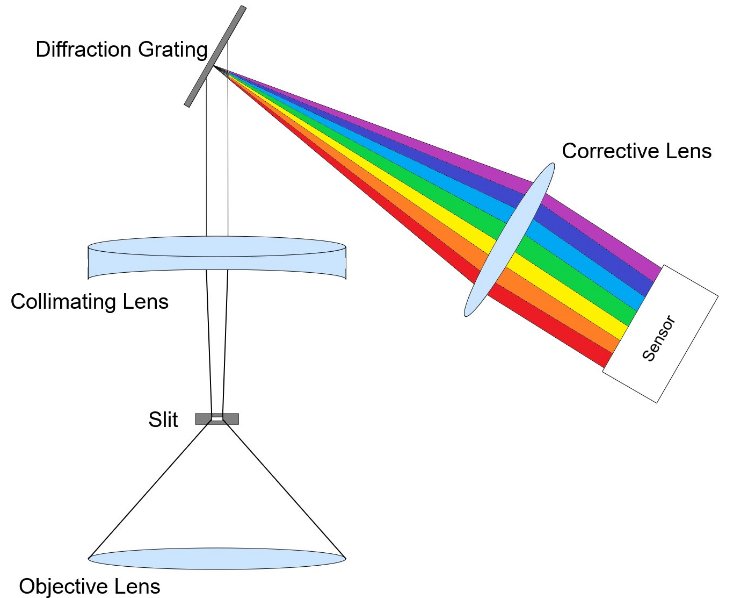
\includegraphics[width=\textwidth]{hsi_optics.png}

            \begin{textblock*}{5cm}(0.2cm,8.5cm)
                \tiny Left image: \cite{hsi-cube} \\ Right image: \cite{nat-presentation}
            \end{textblock*}

            % \vfill
            % {\tiny \hfill Left image: \cite{hsi-cube} \\ \hfill Right image: \cite{nat-presentation}  \par}
        \end{column}
    \end{columns}
\end{frame}

% Note: On this slide mostly want to talk about the images, point out the spectrum and the fact that we get the full spectrum for just one pixel (hence the arrows). The words are not that important
\begin{frame}{Background: HSI for Classification}
    \begin{columns}
        \begin{column}{0.53\textwidth}
            \begin{itemize}
                \item Hyperspectral imaging data can be used to classify objects in images. Their high wavelength spectrum makes them especially useful for environmental monitoring, agriculture, and more.
                \item For our project, we're interested in identifying regions of forests with an adbundance of ground fuel which puts them at risk of forest-fires.
            \end{itemize}


            \begin{textblock*}{5cm}(0.2cm,8.5cm)
                \tiny Top image: \cite{hsi-stones} \\ Bottom image: \cite{hsi-people}
            \end{textblock*}

            % \vfill
            % {\begin{flushleft} \tiny \hfill Top image: \cite{hsi-stones} \\ \hfill Right image: \cite{hsi-people}  \par \end{flushleft}}

        \end{column}
        \begin{column}{0.43\textwidth}
            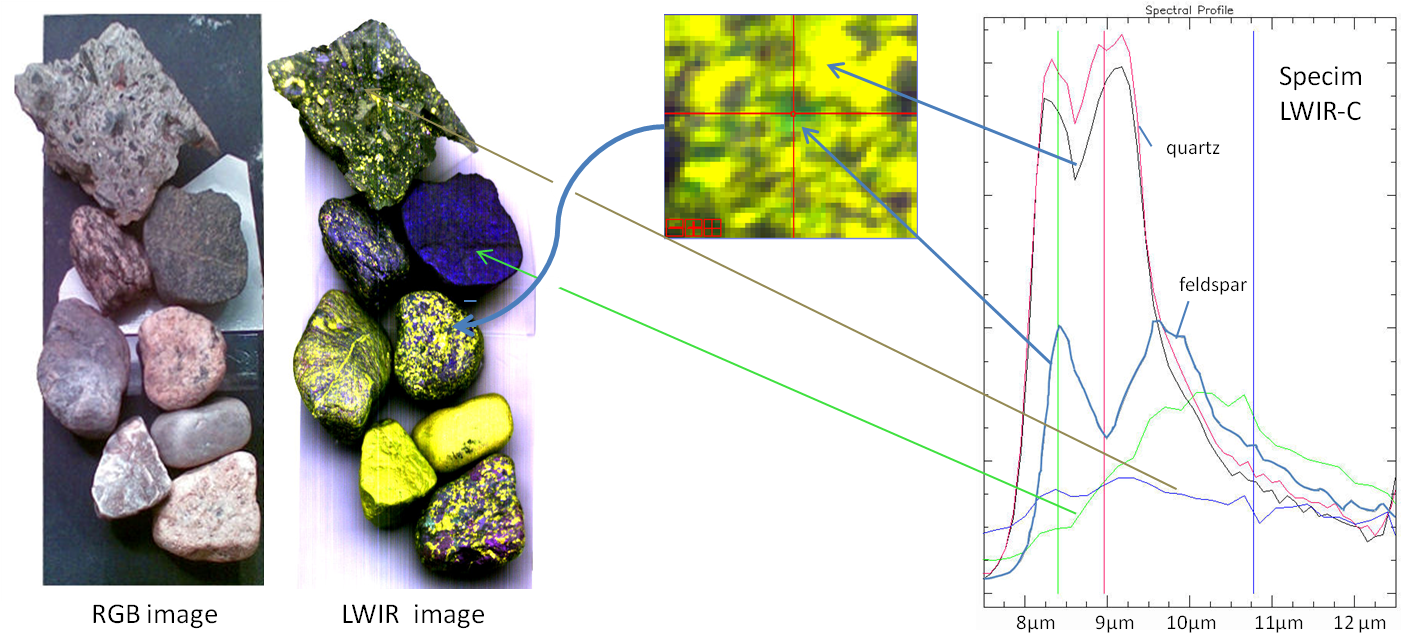
\includegraphics[width=\textwidth]{wiki_hsi2.png}
            \begin{figure}
                \centering
                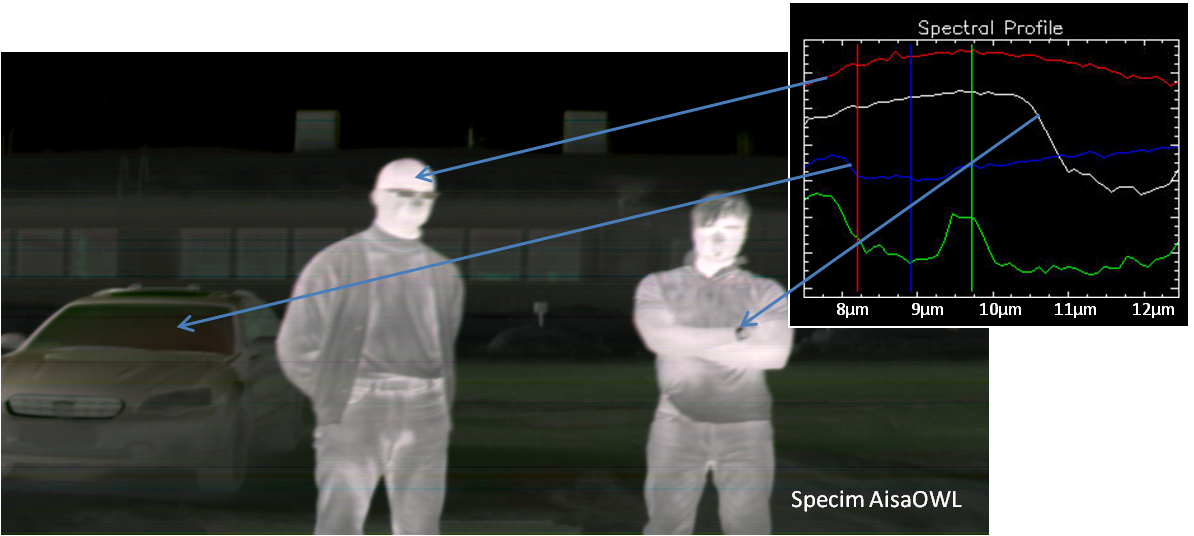
\includegraphics[width=\textwidth]{wiki_hsi1.png}
            \end{figure}
        \end{column}
    \end{columns}
\end{frame}


% Do mention in words the determinism vs nondeterminism of the two approaches (refresh cycles and cache misses), the potential for lower latency for FPGAs due to streaming, the fact that we get programmable i/o
\begin{frame}{Background: FPGAs}
    \begin{itemize}
        \item An \textbf{FPGA} (Field Programmable Gate Array) is a programmable circuit.
        \item They are built out of logic elements, DSP slices (for performing simple addition and multiplication), and local memory (consisting of static RAM).
        \item They consist of a 'fabric' of resources where everything is interconnected (hence programmable).
    \end{itemize}
    \begin{columns}[b]
        \begin{column}{0.48\textwidth}


            \begin{figure}[ht]
                \centering
                \scalebox{0.55} {
                    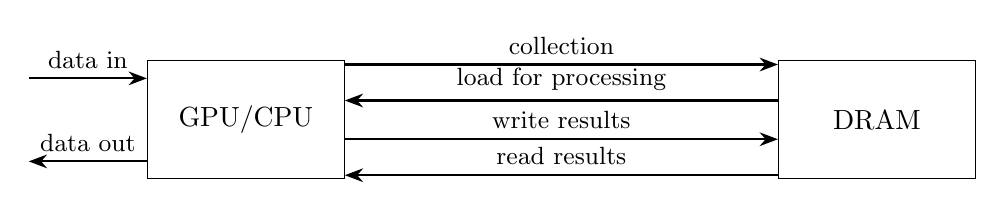
\begin{tikzpicture}[
                        block/.style={rectangle, draw, minimum width=2.5cm, minimum height=1.5cm, align=center},
                        arrow/.style={-{Stealth}, thick},
                        textnode/.style={font=\small}
                        ]

                        % Nodes
                        \node[block] (gpu) {GPU/CPU};
                        \node[block, right=5.5cm of gpu] (dram) {DRAM};

                        \coordinate[left=1.5cm of gpu.west, yshift=15pt] (datain);
                        \coordinate[left=1.5cm of gpu.west, yshift=-15pt] (dataout);

                        % Data in and out arrows
                        \draw[arrow] (datain) -- ([yshift=15pt]gpu.west) node[midway, above, textnode] {data in};
                        \draw[arrow] ([yshift=-15pt]gpu.west) -- (dataout) node[midway, above, textnode] {data out};


                        % Spaced arrows between GPU and DRAM (top to bottom)
                        \draw[arrow] ([yshift=20pt]gpu.east) -- ([yshift=20pt]dram.west) node[midway, above, textnode] {collection};
                        \draw[arrow] ([yshift=7pt]dram.west) -- ([yshift=7pt]gpu.east) node[midway, above, textnode] {load for processing};
                        \draw[arrow] ([yshift=-7pt]gpu.east) -- ([yshift=-7pt]dram.west) node[midway, above, textnode] {write results};
                        \draw[arrow] ([yshift=-20pt]dram.west) -- ([yshift=-20pt]gpu.east) node[midway, above, textnode] {read results};

                    \end{tikzpicture}
                }
                \caption{Latency overhead of using a GPU for computation}
                \label{fig:gpu-diagram}
            \end{figure}
        \end{column}
        \begin{column}{0.48\textwidth}
            \begin{figure}[ht]
                \centering
                \scalebox{0.55} {
                    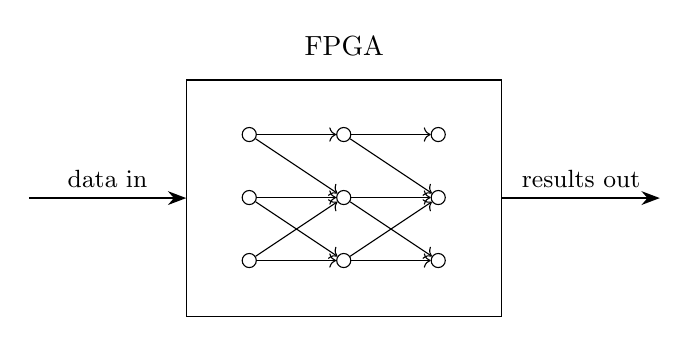
\begin{tikzpicture}[
                        block/.style={rectangle, draw, minimum width=4cm, minimum height=3cm, align=center},
                        arrow/.style={-{Stealth}, thick},
                        nodecircle/.style={circle, draw, fill=white, inner sep=1.8pt},
                        textnode/.style={font=\small}
                        ]

                        % FPGA block
                        \node[block] (fpga) {};
                        \node[above=5pt of fpga.north] {FPGA};

                        % Input and output coordinates
                        \coordinate[left=2cm of fpga.west] (datain);
                        \coordinate[right=2cm of fpga.east] (resultsout);

                        % Data in and results out arrows
                        \draw[arrow] (datain) -- (fpga.west) node[midway, above, textnode] {data in};
                        \draw[arrow] (fpga.east) -- (resultsout) node[midway, above, textnode] {results out};

                        % Define circle positions inside FPGA block in 3 vertical layers
                        \foreach \layer/\x in {1/0.8, 2/2.0, 3/3.2} {
                                \foreach \row/\y in {1/0.7, 2/1.5, 3/2.3} {
                                        \node[nodecircle] (c\layer\row) at ([shift={(\x cm,-\y cm)}]fpga.north west) {};
                                    }
                            }

                        % Arrows from layer 1 to layer 2 (mixed connections)
                        \draw[->] (c11) -- (c21);
                        \draw[->] (c11) -- (c22);
                        \draw[->] (c12) -- (c22);
                        \draw[->] (c12) -- (c23);
                        \draw[->] (c13) -- (c22);
                        \draw[->] (c13) -- (c23);

                        % Arrows from layer 2 to layer 3 (mixed connections)
                        \draw[->] (c21) -- (c31);
                        \draw[->] (c21) -- (c32);
                        \draw[->] (c22) -- (c32);
                        \draw[->] (c22) -- (c33);
                        \draw[->] (c23) -- (c32);
                        \draw[->] (c23) -- (c33);

                    \end{tikzpicture}
                }
                \caption{Lack of latency overhead of an FPGA inference stream}
                \label{fig:fpgadiagram}
            \end{figure}
        \end{column}
    \end{columns}
\end{frame}


\begin{frame}{Research Question}
    \begin{alertblock}{Research Question}
        How much can different neural network model architectures for classifying hyperspectral data improve latency in an FPGA implementation without sacrificing accuracy?
    \end{alertblock}
    \myheading{Baseline}
    \begin{itemize}
        \item Previous work at MSU successfully reduced band dimension on a HSI dataset and performed high accuracy classification on it.
        \item 99.7\% accuracy using a large convolutional neural network.
        \item Performs roughly 2 billion elementary add/multiply operations for each pixel classified.
    \end{itemize}
\end{frame}

\begin{frame}
    \begin{figure}
        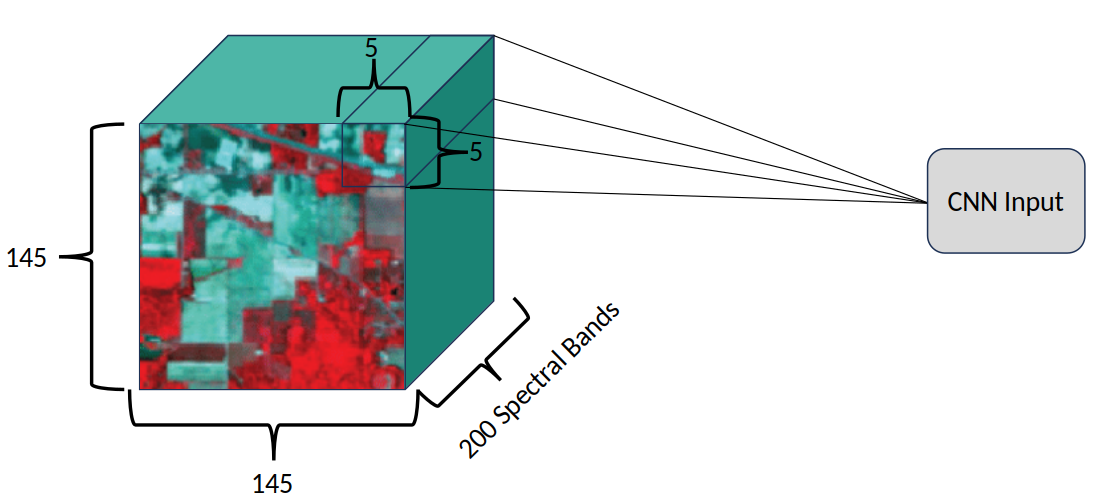
\includegraphics[width=0.5\linewidth]{cnn_data.png}
        % 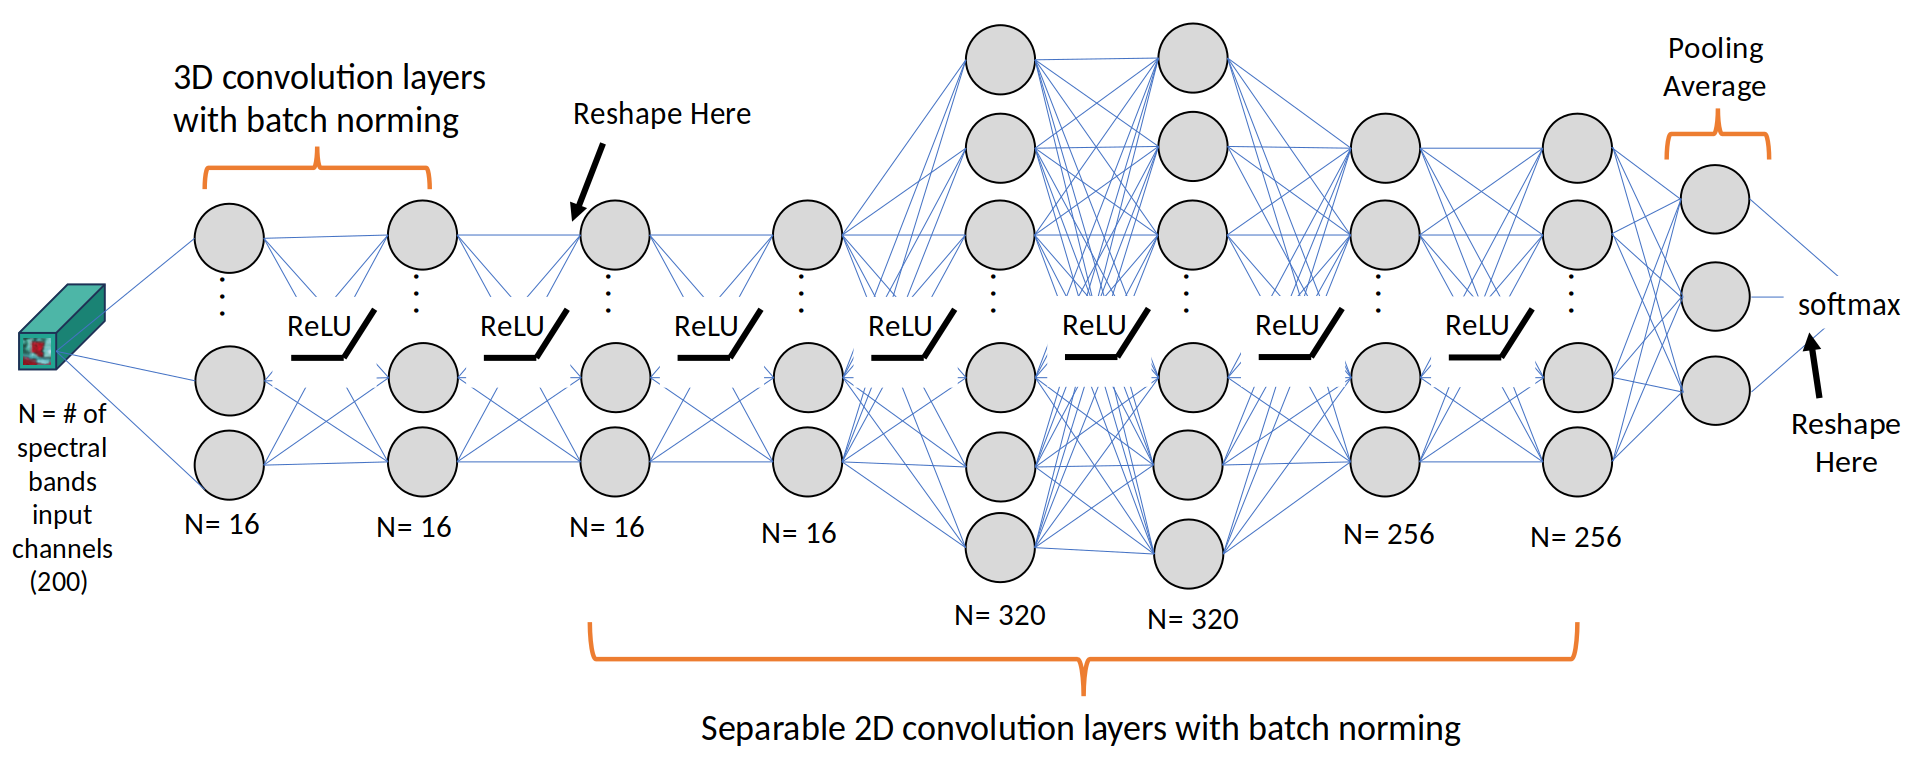
\includegraphics[width=0.7\linewidth]{cnn_arch.png}
    \end{figure}

    \begin{figure}
        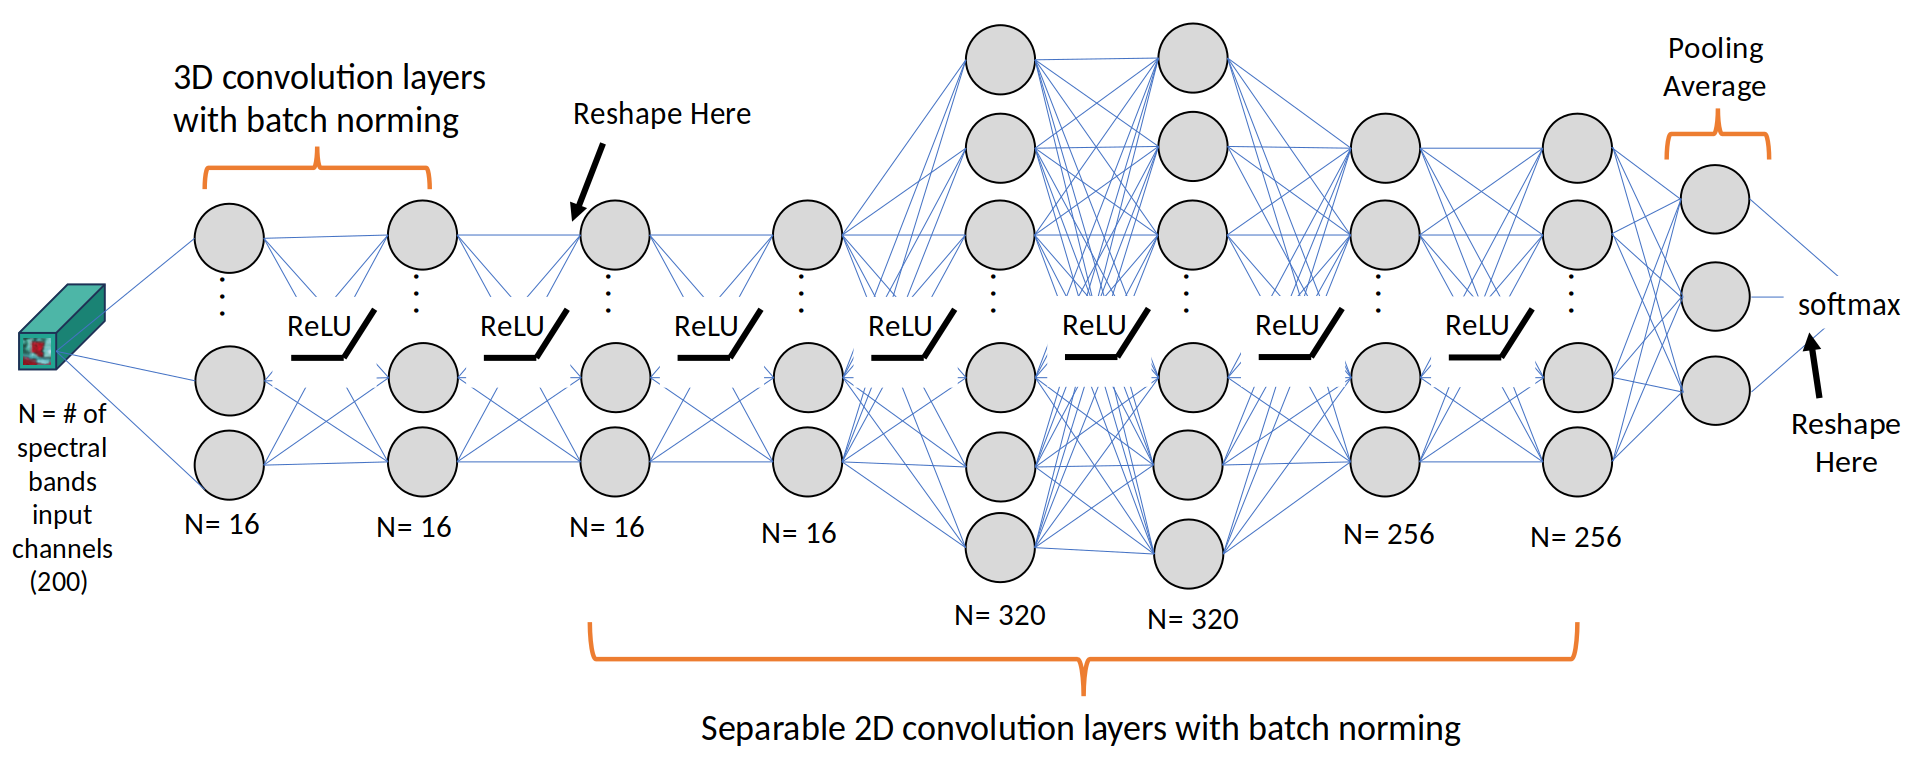
\includegraphics[width=0.8\linewidth]{cnn_arch.png}
    \end{figure}

    \begin{textblock*}{5cm}(0.2cm,8.5cm)
        \tiny Both images: \cite{dirk-presentation}
    \end{textblock*}

\end{frame}

% Note that the discussion of CNN drawbacks is kinda irrelevant now that
% we're loading data anyways. May want to adjust this section
\begin{frame}{Alternative Architectures}
    \myheading{CNN Drawbacks}
    \begin{itemize}
        \item A CNN allows us to gain spatial information about our image by taking into account pixels around each pixel
              \begin{itemize}
                  \item For real time classification, this requires storing data so our kernel can pass over it, interrupting the flow of data through our FPGA
              \end{itemize}
        \item The CNN implementations are also quite large and might not be viable for our hardware needs.
    \end{itemize}


    \myheading{Kolmogorov Arnold Networks (KAN)}
    % This is probably the section that I need to say the most in words. In particular, explain the differences between
    % Fixed activation + linear transformation in a traditional MLP vs learning activations directly
    \begin{itemize}
        \item Directly learns the nonlinear activation functions of a network.
        \item In an FPGA, these functions could be encoded directly as \textbf{lookup tables}, allowing us to approximate results much more quickly.
        \item If pixel-classification is viable, we can avoid storing/transferring data from memory for a CNN kernel.
    \end{itemize}
\end{frame}

\begin{frame}
    \begin{figure}
        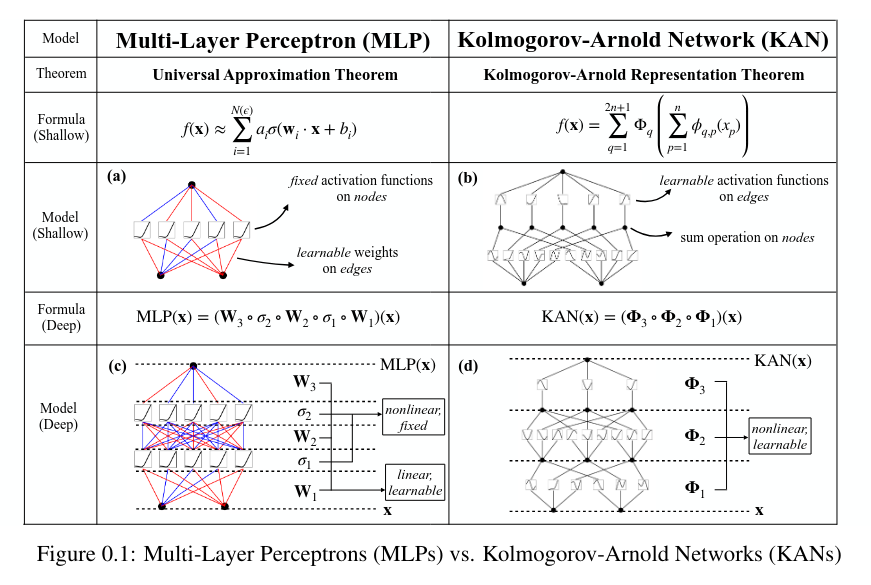
\includegraphics[width=0.75\linewidth]{mlpkan.png}
    \end{figure}


    \begin{textblock*}{5cm}(0.2cm,8.5cm)
        \tiny Image: \cite{kan}
    \end{textblock*}

\end{frame}

\begin{frame}{More on Lookup Tables}

    \begin{itemize}
        \item Each lookup table consists of both the actual stored values as well as the meta-data necessary do our lookups.
    \end{itemize}


    \begin{columns}[t]
        \column{0.48\textwidth}
        \begin{adjustbox}{width=\textwidth}
            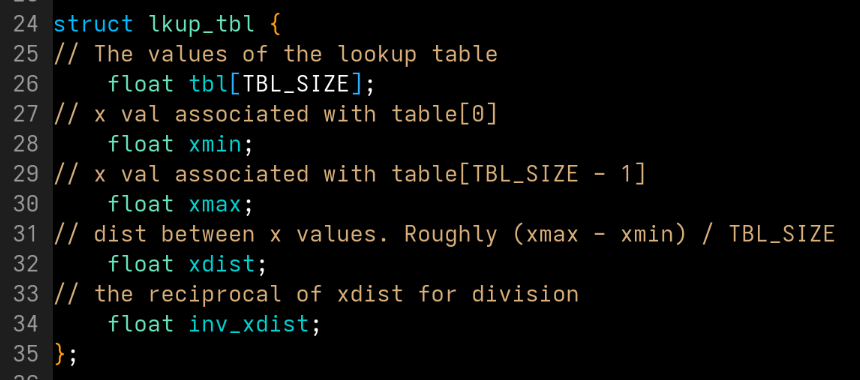
\includegraphics{lkuptblcode.png}
        \end{adjustbox}

        \column{0.48\textwidth}
        \begin{adjustbox}{width=\textwidth}

            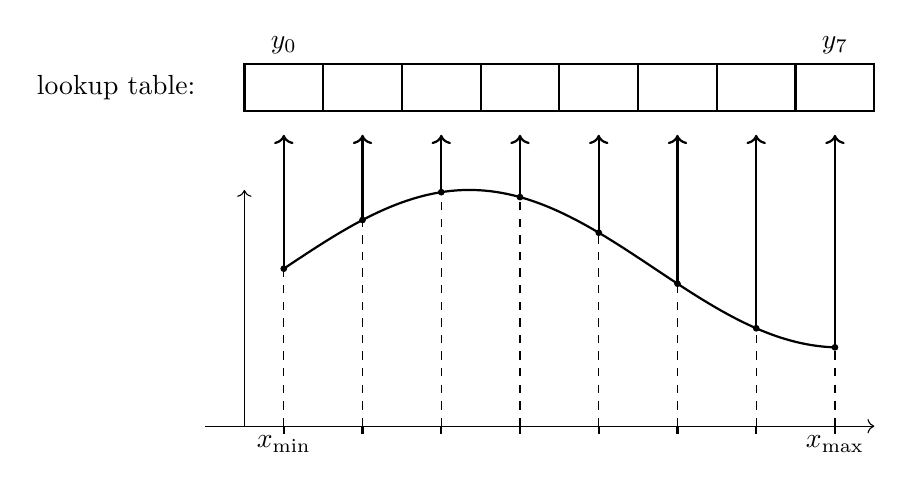
\begin{tikzpicture}

                % Parameters
                \def\npoints{8}
                \def\tableHeight{4}
                \def\boxWidth{1}
                \def\xstart{1} % Starting x-value (instead of 0)
                \def\xend{8}   % 8 intervals = 9 points

                % Axes
                \draw[->] (\xstart - 1, 0) -- (\xend + 0.5, 0); % x-axis
                \draw[->] (\xstart - 0.5, 0) -- (\xstart - 0.5, 3); % y-axis

                % Function and evaluation points
                \foreach \i in {0,...,7} {
                        \pgfmathsetmacro\x{\xstart + \i}
                        \pgfmathsetmacro\y{2 + sin(deg((\x - 1)/1.5))} % offset for natural xmin
                        \filldraw[black] (\x,\y) circle (1pt);  % function evaluation point
                        \draw[dashed] (\x,0) -- (\x,\y);       % dashed vertical line
                        \draw[->, thick] (\x,\y) -- (\x,\tableHeight - 0.3); % arrow to table
                        \draw[thick] (\x,0) -- ++(0,-0.1);     % x-axis tick mark
                    }

                % Draw the function curve
                \draw[thick, smooth, domain=\xstart:\xend, samples=100]
                plot(\x, {2 + sin(deg((\x - 1)/1.5))});

                % Lookup table boxes (aligned with center of evaluation points)
                \foreach \i in {0,...,7} {
                        \pgfmathsetmacro\x{\xstart + \i - 0.5}
                        \draw[thick] (\x, \tableHeight) rectangle ++(\boxWidth, 0.6);
                    }

                % Labels
                \node[below] at (\xstart, 0) {$x_{\min}$};
                \node[below] at (\xend, 0) {$x_{\max}$};
                \node[above] at (\xstart + 0.0, \tableHeight + 0.6) {$y_0$};
                \node[above] at (\xend - 0.0, \tableHeight + 0.6) {$y_7$};
                \node[left] at (\xstart - 1, \tableHeight + 0.3) {lookup table:};
            \end{tikzpicture}

        \end{adjustbox}
    \end{columns}

    % Note: this is kinda different than the sort of loading for a CNN because the CNN requires we first stream/write data to memory and then load it into the fpga which complicates pipelining and kinda inherently adds latency (at least for a single pixel -- might not affect overall throughput?), but with lookup tables we still stream data directly and just need to pipeline the loading properly so it gets there 
    \begin{itemize}
        \item Thus to do a lookup on our table, we use \texttt{xmin}, \texttt{xmax}, \texttt{xdist}, and \texttt{inv\_xdist} to do linear interpolation between the lookup table entries nearest to our input.
        \item These lookup tables take up a significant amount of memory -- much more than is available locally in our FPGA.
    \end{itemize}


\end{frame}


% Note that I'm neglecting to mention this work in final presentation, thus should allude to it (?)

% \begin{frame}{Work Done}
%   \begin{itemize}
%     \item To properly benchmark and implement, we need to shift the models from the high level and opaque python implementations to something lower level.
%     \item To do this, I transferred both the baseline CNN implementation and the KAN to C (for the latter, I created a custom C library that can be called directly from python).
%           \begin{itemize}
%             \item This allows us to do preliminary benchmarking and provides an interface to swap out the computational parts of the classification directly to the FPGAs.
%             \item This process will likely form the basis of the rest of my work at the REU.
%           \end{itemize}

%   \end{itemize}
% \end{frame}


% Additional Slides:
% Note: I only have 5 more minutes than last time
% Emphasize lookup tables in previous slides. Remove information as much as possible/go faster in explanation
% Future slides:
% Device driver motivation
% Device driver design
% Device driver implementation
% And lowkey call it a day there

% Say something along the lines of "Work on the device driver constituted pretty much the entirety of my work for the second half of the REU"
\begin{frame}{Device Driver Introduction and Motivation}

    % words
    \begin{columns}
        \column{0.53\textwidth}
        \begin{itemize}
            \item A \textbf{device driver} is a piece of software that provides an interface between an operating system and the hardware devices it runs on.
            \item We want to write a driver that can transfer large amounts of data from system memory (DRAM) to local fabric memory (SRAM) on the FPGA efficiently.
        \end{itemize}
        \column{0.43\textwidth}
        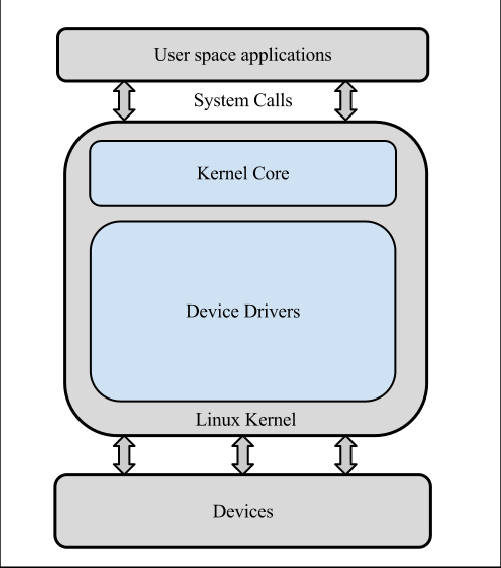
\includegraphics[scale=0.6]{kerneltree.png}
    \end{columns}

    \begin{textblock*}{5cm}(0.2cm,8.5cm)
        \tiny Image: \cite{kernel-tree}
    \end{textblock*}

\end{frame}

\begin{frame}{Device Driver Design}

    \begin{columns}
        \column{0.43\textwidth}
        \begin{itemize}
            \footnotesize
            \item Significant portions of our board's address space are reserved for data buses and peripheral devices.
                  \begin{itemize}
                      \footnotesize
                      \item Thus we can use our driver to write to a portion of the address space that corresponds to a data bus accessible to our FPGA.
                  \end{itemize}
            \item A \textbf{device tree} in Linux describes the components of the hardware that Linux is running on.
            \item We create two entries in our device tree corresponding to addresses accessible to the FPGA through an AXI bus. The bus connects to seperate ports in the static RAM of our FPGA.
        \end{itemize}
        \column{0.57\textwidth}

        \begin{figure}
            \centering

            \begin{adjustbox}{width=\textwidth}
                \begin{circuitikz}
                    \tikzstyle{every node}=[font=\normalsize]
                    \draw  (2,11.5) rectangle (4,10.5);
                    \draw  (5,12.5) rectangle (7,11.5);
                    \draw  (5,10.5) rectangle (7,9.5);
                    \draw [->, >=Stealth] (4,11) -- (5,12);
                    \draw [->, >=Stealth] (4,11) -- (5,10);
                    \node [font=\normalsize] at (3,11) {User};
                    \node [font=\normalsize] at (6,12) {Driver B};
                    \node [font=\normalsize] at (6,10) {Driver A};
                    \draw  (9,14.5) rectangle (10.75,6.25);
                    \draw [short] (9,12) -- (10.75,12);
                    \draw [short] (9,9.25) -- (10.75,9.25);
                    \draw [->, >=Stealth] (7,12) -- (9,10.75);
                    \draw [->, >=Stealth] (7,10) -- (9,9.25);
                    \draw [dashed] (9,10.75) -- (10.75,10.75);
                    \draw [short] (11.5,12) -- (11.5,7.75);
                    \draw [short] (11.25,9.25) -- (11.75,9.25);
                    \draw [short] (11.25,12) -- (11.75,12);
                    \draw [->, >=Stealth] (11.5,7.75) -- (14.5,7.75);
                    \draw  (15.5,8.5) rectangle (16.75,6.25);
                    \draw [<->, >=Stealth] (14.5,7.75) -- (15.5,7.75);
                    \draw [dashed] (15.5,7.75) -- (16.75,7.75);
                    \draw [dashed] (15.5,7) -- (16.75,7);
                    \node [font=\normalsize] at (10,15.25) {Physical Address Space};
                    \node [font=\normalsize] at (16,8.75) {SRAM};
                    \node [font=\tiny] at (13,12) {0x0047\_FFFF\_FFFF};
                    \node [font=\tiny] at (13,10.75) {$0x0030\_0000\_0000$};
                    \node [font=\tiny] at (13,9.25) {0x0010\_0000\_0000};
                    \node [font=\normalsize] at (12.5,14.5) {0x0100\_0000\_0000};
                    \node [font=\normalsize] at (11.25,6.25) {0x0};
                    \node [font=\normalsize] at (15,8) {A/B};
                    \node [font=\small] at (12.5,7.5) {M\_AXI\_HPM0\_FPD};
                \end{circuitikz}
            \end{adjustbox}
        \end{figure}
    \end{columns}

\end{frame}

\begin{frame}{Device Driver Implementation}
    Write this when done, or scrap it if I get cooked :(

\end{frame}

\begin{frame}{Future Work}
    \begin{itemize}
        \item KAN accuracy tradeoffs with different lookup table sizes and data type precisions.
        \item Model pruning.
        \item Benchmarking C implementations on the FPGA.
        \item Device driver latency overhead and pipelining. %, considering that 
        % \begin{itemize}
            % \item Given that multiple batches of lookup tables will need to be loaded and unloaded in the course of a single inference pass.
        % \end{itemize}
        \item Direct Memory Access (DMA) Implementation.
    \end{itemize}
    \centering
    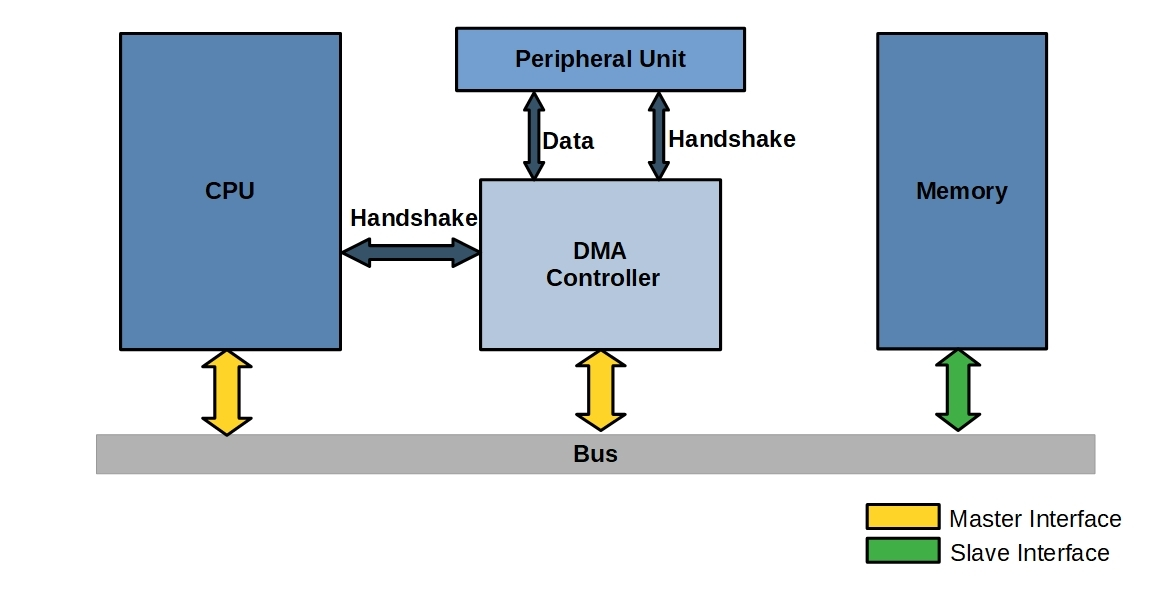
\includegraphics[scale=0.17]{dma-diagram.jpg}

    \begin{textblock*}{5cm}(0.2cm,8.5cm)
        \tiny Image: \cite{dma}
    \end{textblock*}
    
    
\end{frame}


% Modify this conclusion significantly
\begin{frame}{Conclusion}
    \myheading{Project Summary}
    \begin{itemize}
        \item This project began as an investigation of model architectures that would be suitable for hyperspectral classification on an FPGA.
        \item As it progressed, it became clear that a significant bottleneck for a real implementation would be loading data onto an FPGA, so I created a device driver that could accomplish that.
    \end{itemize}

    % \myheading{Highlights}
    % \begin{itemize}
    %   \item I've enjoyed looking into ML implementations at a lower level and I'm excited to begin swapping out some of my implementations with real FPGA hardware.
    % \end{itemize}

    \begin{block}{Summary}
        Our goal is to achieve real-time HSI classification using a custom FPGA implementation. The real-time nature of this implementation would be highly useful for field work and real applications, but requires overcoming engineering challenges related to our hardware.
    \end{block}
\end{frame}


\begin{frame}{Acknowledgements}
    \begin{itemize}
        \item This material is based upon work supported by the National Science Foundation under Grant No. 2349091.
        \item I would like to acknowledge my PI Ross Snider for the direction and assistance he has provided on the project.
        \item I would also like to thank Nat Sweeney, Zackery Backman, and Dirk Kaiser for the work that they have done and continue to do on the project.
        \item And a special thank you to my peers in the REU program that have made this summer fun and memorable for me, and for the support and encouragement they have provided throughout the summer.
    \end{itemize}
\end{frame}


% I think I just need to add citations for the presentations I was shown (and tbh this is optional)
\begin{frame}[allowframebreaks]{References}
    \begingroup
    \tiny
    \setlength{\itemsep}{0pt}
    \setlength{\parsep}{0pt}
    \setlength{\parskip}{0pt}
    \nocite{*}
    % \setlength\bibitemsep{0.3ex}
    % \printbibliography[heading=none]
    \bibliographystyle{acm}
    \bibliography{reference.bib}
    \endgroup
\end{frame}

\begin{frame}
    \Huge{\centerline{\textbf{The End}}}
\end{frame}

\end{document}
